\documentclass{article}
\usepackage{PRIMEarxiv}
\usepackage[T1]{fontenc}
\usepackage[utf8]{inputenc}
\usepackage{amsmath,amssymb,booktabs,tabularx,array,graphicx,microtype,hyperref}
\hypersetup{hidelinks,pdftitle={How Much Teammate Information Is Needed for Decentralized Fine Alignment of Two Robot Arms?},pdfauthor={Group 28, IIT Gandhinagar}}
\graphicspath{{media/}}
\fancyhead[L]{\small\itshape Decentralized Dual-Arm Fine Alignment}
\fancyhead[R]{\small Group 28 --- Multi-Agent Systems}
\setlength{\emergencystretch}{1.5em}
\setlength{\tabcolsep}{5pt}
\raggedbottom
% Generated from the verified episode analyses. Do not hand-edit numerical cells.
\newcommand{\LocalGap}{1.1}
\newcommand{\LocalCost}{2.356}
\newcommand{\OracleCost}{2.331}
\newcommand{\CapPayload}{152.4}
\newcommand{\BidPayload}{76.2}
\newcommand{\RgbAlignRange}{99.2--99.9}
\newcommand{\LearnedContactRange}{68.0--79.7}
\newcommand{\HalfInserted}{104}
\newcommand{\TruthInserted}{118}
\newcommand{\ContactDiff}{-21.9}
\newcommand{\ContactDiffCI}{-30.5, -14.1}
\newcommand{\BlockedInserted}{0}
\newcommand{\BlockedN}{64}
\newcommand{\BlockedReleased}{53}
\newcommand{\BlockedTried}{53}
\newcommand{\OpenReleased}{1}
\newcommand{\OpenTried}{11}
\newcommand{\LearnedPreFail}{151}
\newcommand{\LearnedDescentFail}{44}
\newcommand{\LearnedHoldFail}{1}
\newcommand{\LearnedPoseReject}{143}
\newcommand{\LearnedVisionReject}{8}
\newcommand{\AlignmentRows}{%
\multicolumn{5}{@{}l}{\textit{Deterministic allocation references (GT only)}} \\
S0 joint reference & 100.0 & 2.331 & -- & -- \\
S1 local model & 100.0 & 2.356 & -- & -- \\
Fixed half & 100.0 & 3.757 & -- & -- \\
\midrule
\multicolumn{5}{@{}l}{\textit{Learned policies: same frozen actor under GT and RGB}} \\
PPO S1 & 100.0 & 5.668 & 99.2 & 8.570 \\
PPO S2 & 100.0 & 4.645 & 99.6 & 5.908 \\
PPO S3 & 100.0 & 5.498 & 99.9 & 7.912 \\
PPO S4 & 100.0 & 5.309 & 99.5 & 7.402 \\
}
\newcommand{\FailureRows}{%
Learned RGB (six conditions) & 768 & 151 & 44 & 1 & 572 \\
Fixed-half RGB & 128 & 18 & 6 & 0 & 104 \\
S1 / ground truth & 128 & 0 & 10 & 0 & 118 \\
}

% Confirm with the group before upload. Replace the four values with factual status.
\newcommand{\GauravStatus}{\textemdash}
\newcommand{\AayushStatus}{\textemdash}
\newcommand{\LaxmidharStatus}{\textemdash}
\newcommand{\RoshinStatus}{\textemdash}
% Replace after publication, e.g. \renewcommand{\RepositoryLink}{\href{...}{Group 28 repository}}.
\newcommand{\RepositoryLink}{To be provided by the group with submission.}

\title{How Much Teammate Information Is Needed for\texorpdfstring{\\}{ }Decentralized Fine Alignment of Two Robot Arms?}
\author{Gaurav Srivastava \quad Aayush Bundel \quad Laxmidhar Swine \quad Roshin Gelasious\\[.4em]
Indian Institute of Technology Gandhinagar\\
Foundations of AI: Multiagent Systems \enspace $\cdot$ \enspace Group 28}

\begin{document}
\maketitle
\thispagestyle{empty}
\begin{abstract}
Two robot arms can correct the same peg--fixture alignment error, but each may have a different motion cost and limited knowledge of the other's decision. We compare local rules, capability messages, history-based prediction and pre-action bids against a full-information allocator. Across 1,000 matched test cases for the first fitted model, the strongest no-message rule succeeds on every case and comes within \LocalGap\% of the reference on mean squared joint motion. A compact capability exchange closes that small gap in this model; richer information does not reliably improve results. We train decentralized PPO actors and integrate neural RGB sensing, then evaluate transfer to motor-driven, force-controlled insertion. Learned RGB policies align on \RgbAlignRange\% of core starts, but insert on \LearnedContactRange\% across the learned RGB open-hole conditions and do not beat the fixed-half RGB controller on insertion motion cost. The results separate the benefits of an allocation convention, teammate information, and perception accuracy.
\end{abstract}
\keywords{cooperative decision-making \and communication-limited coordination \and multi-agent reinforcement learning \and peg-in-hole assembly}

\section{Introduction}
When a peg sits 4\,mm to the right of a receiving hole, the peg arm can move left, the receiver arm can move right, or both can share the correction. These choices can yield the same relative pose but not the same joint movement: one robot may be near a less favorable configuration. If each robot independently commands the full correction both can overshoot; if both wait for the other, the error persists. This is an allocation problem before it is an insertion problem.

The distinction between \emph{capability} and \emph{intent} matters. A compact summary of a teammate's kinematic costs tells an agent which motion is cheaper for that teammate, not whether the teammate will actually choose it. Conversely, a pre-action bid describes intended effort but depends on the convention that translates bids into motions. We ask how much each extra information source helps when the two decisions must be made without a centralized action selector.

\textbf{Research questions.} Can a strong local rule approach a joint allocator without sending messages? How do a current capability summary, a prediction from past motion, and a current bid trade off payload and executed motion? Finally, does coordination learned for planar alignment remain useful when the estimate comes from RGB and the parts make physical contact in simulation?

\textbf{Study design.} We first compare methods with a matched ground-truth observation so that the allocation question is not confounded by camera error. We then cross learned policies with ground-truth and neural RGB sensing. A separate dynamic study evaluates insertion after alignment, rather than treating alignment success as proof of assembly.

\clearpage
\subsection{Origin and scope}
Our work builds on the Seam Filling Network of Xie et al.\ \cite{xie}: segment the peg and seam, estimate relative lateral translation and yaw, and use the estimates in a visual feedback loop. The published physical-robot results are those of Xie et al., not ours. Before this course project, Gaurav Srivastava implemented and studied the single-arm pipeline in simulation for his MTech thesis under Prof. Harish P M \cite{sfnsystem}. He discussed the proposed continuation with the course instructor, Prof. Manisha Padala, before submitting the project idea.

That earlier work answers \emph{what correction should one arm execute?} The course project asks \emph{which of two arms should produce each part of a correction?} We reuse relevant Panda and perception infrastructure, including the segmentation architecture and its starting weights. New course work comprises the shared two-arm environment, local information protocols and cost-aware comparisons, cooperative policy training, adaptation of the visual estimator to a moving receiver, and a paired evaluation of alignment and dual-arm contact assembly. Prior single-arm results are background, not evidence for any of the new controllers.

\begin{figure}[!ht]
\centering
\begin{minipage}[t]{.48\linewidth}\centering
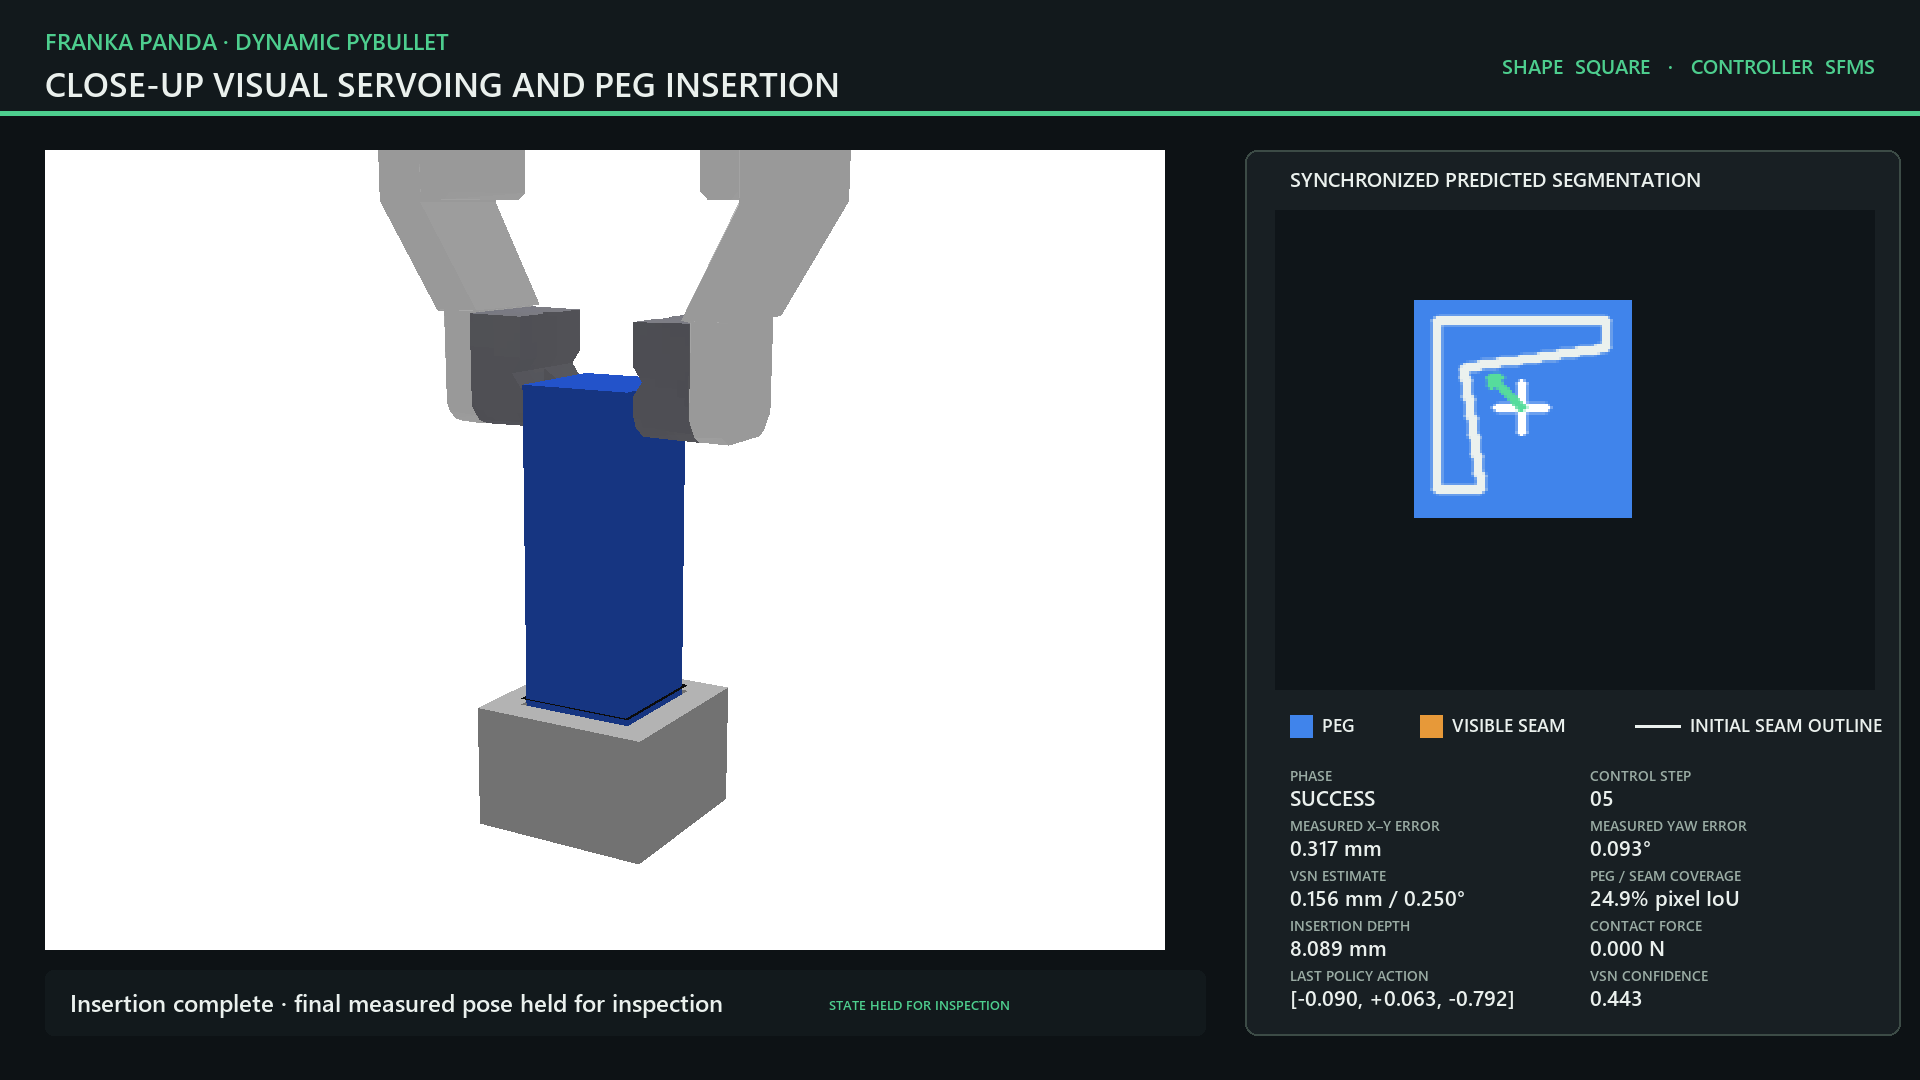
\includegraphics[width=\linewidth,height=1.72in,keepaspectratio]{single-arm.png}\\[-.1em]
\small (a) Prior MTech thesis: single-arm simulation
\end{minipage}\hfill
\begin{minipage}[t]{.48\linewidth}\centering
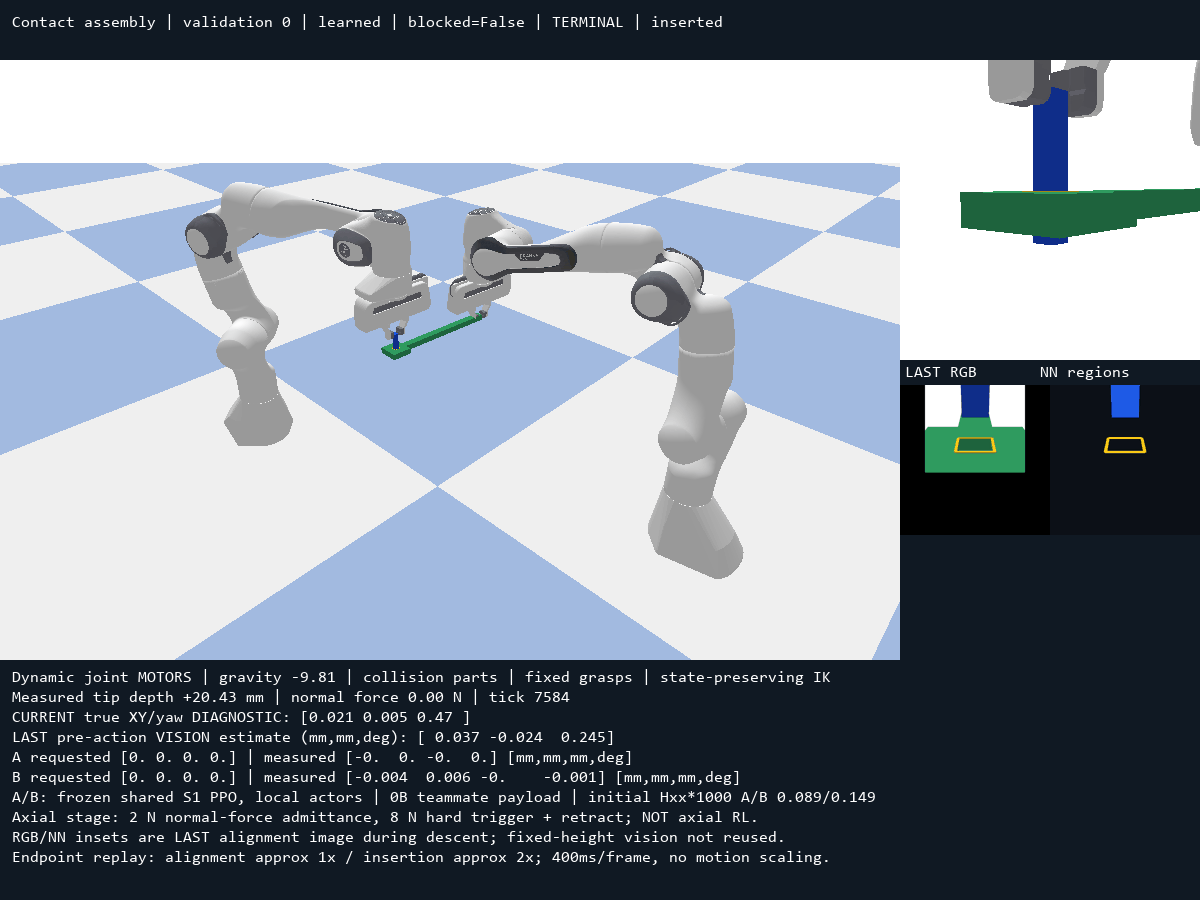
\includegraphics[width=\linewidth,height=1.72in,keepaspectratio]{dual-arm.png}\\[-.1em]
\small (b) Course study: both parts held and controlled
\end{minipage}
\caption{Prior single-arm SFN implementation (a) and an executed RGB-to-insertion replay from this course project (b). Neither image shows hardware. The full replay and frame sources are in the bundle.}
\label{fig:lineage}
\end{figure}

\section{Preliminaries}
Let $A$ hold the peg and $B$ hold the fixture. The task error $e=(\Delta x,\Delta y,\Delta\psi)^\top$ is peg minus fixture in a common world frame; translations are in metres and wrapped yaw in radians. Each arm has seven joints $q_i$ and produces a signed increment $a_i$ of its own held reference point. Identical translations cancel in relative error. For sufficiently small moves, $e^+\simeq\operatorname{wrap}_\psi(e+a_A-a_B)$, but the simulator measures the executed held transforms to evaluate $e^+$ instead of assuming this identity holds exactly.

\section{Problem formulation}
A centralized reference observes both configurations and jointly assigns corrections; a local actor sees the common sensed error, its own joints and cost, and only the extra information permitted by its regime. This is a cooperative partially observed decision problem \cite{bernstein}: rewards are shared, but observations need not be. With global state $s_t=(e_t,q_{A,t},q_{B,t})$ and available local history $h_{i,t}$, each action is selected by $\pi_i(a_i\mid h_{i,t})$. The learned team maximizes $\mathbb E[\sum_{t<T}\gamma^t r_t]$ subject to per-arm feasible actions and the information restrictions of Table~\ref{tab:protocol}. Alignment ends at $|\Delta x|,|\Delta y|\leq 1$\,mm and $|\Delta\psi|\leq 1^\circ$, or after 20 commands. Insertion is scored separately.

\clearpage
\section{Methodology}
\subsection{Measured world, allocation, and information}
A single PyBullet simulation instance manages both Panda robot models. Both policies observe the same pre-step state before either motion executes (Fig.~\ref{fig:workflow}). The alignment benchmark uses full-pose inverse kinematics (IK) and joint interpolation, not contact physics. Per-arm limits are 2\,mm per lateral axis and 0.04\,rad yaw per command. Joint, IK and sampled collision constraints reject infeasible actions. Outcomes use measured, not requested, error.

\begin{figure}[!ht]
\centering
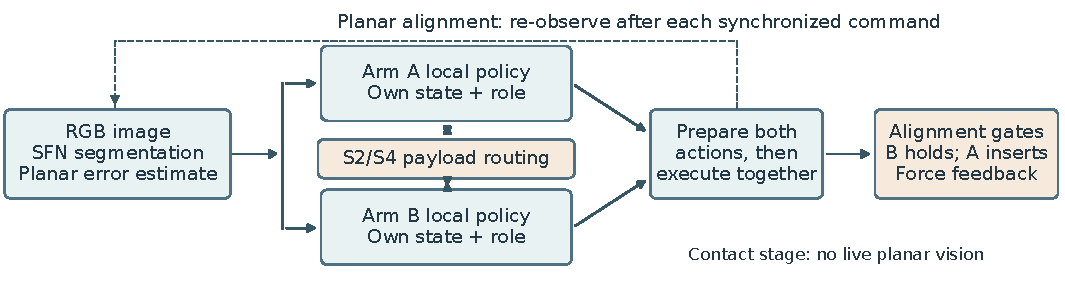
\includegraphics[width=\linewidth]{workflow.pdf}
\caption{Execution workflow. S1/S3 need no teammate messages; S2/S4 route permitted payloads before action selection. The GT comparison substitutes true planar error for the image estimate. Contact insertion begins only after alignment and pose checks.}
\label{fig:workflow}
\end{figure}

For normalized local increment $u_i$, constrained IK gives $\Delta q_i \approx D_i u_i$. Finite differences at the held reference point estimate $D_i$, with full-pose constraints maintained. $H_i=D_i^\top D_i$ predicts squared joint displacement; measured cost is
\begin{equation}
    C = \sum_{t,i}\lVert q_{i,t+1}-q_{i,t}\rVert_2^2 .
    \label{eq:cost}
\end{equation}
This is not energy: dividing a move into smaller commands can lower the sum. Joint travel, commands, terminal error and payload are also recorded.

\begin{table}[!ht]
\centering
\caption{Information available before execution; common sensing is excluded from payload.}
\begin{tabularx}{\linewidth}{@{}lXl@{}}
\toprule
Regime & Rule or additional information & Payload per command \\ \midrule
S0 & Joint cost allocation using both arms' capability. & Not decentralized \\[2pt]
S1 & Own cost plus a public cost prior: a shared model fitted before testing. & 0 bytes \\[2pt]
S2 & Other arm's symmetric $3\times3$ local cost matrix. & 48 bytes, one round \\[2pt]
S3 & Belief from past shared error changes and own executed motion. & 0 bytes \\[2pt]
S4 & Independent public local-model bids, routed before final actions. & 24 bytes, one round \\
\bottomrule
\end{tabularx}
\label{tab:protocol}
\end{table}

\textbf{References and controls.} One-arm-only and fixed-half methods divide the same correction. S0 minimizes one-step predicted cost on a finite grid, not global trajectory cost. S1 substitutes its public prior for current teammate capability; S2 receives that capability instead. S3 combines a fitted prior and four past transitions in an expected-loss search. Its \emph{fixed-belief control} uses the identical solver without updating from history. S4's independent bids change reconciliation as well as information.

Float32 payload includes dropped transmissions but excludes headers and common sensing. All fitted models face the same held-out initial conditions. Each development/model seed pair defines a \emph{fit}; \emph{fit 0} is the first. This term does not denote a separate test set.

\textbf{Why S2 can match S0.} Let $c=\operatorname{clip}(e/s,-1,1)$ with $s=(.002,.002,.04)$. A 125-point grid of $f\in\{0,.25,.5,.75,1\}^3$ produces $u_A=-f\odot c$ and $u_B=(1-f)\odot c$. Both S2 agents reconstruct the objective $u_A^\top H_Au_A+u_B^\top H_Bu_B$ and agreed tie-break rule from the two matrices. Execution is decentralized, but the allocation convention is shared in advance; this does not solve unknown intent in general.

S3 reconstructs past, not current, teammate motion: $\widehat a_B=a_A^{\rm exec}-(e^+-e)$ for A, with wrapped yaw. Observation noise affects this belief. Unlike the allocation grid, its independently chosen shares need not sum to one correction.

\clearpage
\subsection{Cooperative PPO and visual observations}
The learned method uses centralized training and decentralized execution \cite{ppo,mappo}. One shared, role-conditioned actor has 39 inputs and two 64-unit hidden layers. For each axis it selects a correction fraction from $\{0,.25,.5,.75,1\}$. Arm $A$ acts opposite to the clipped sensed error and arm $B$ in the same direction, each scaled by its own fraction. Thus the action space permits unequal contributions and over- or under-correction; the geometric scaffold supplies the direction but not a joint action split. Missing information slots are zero.

A separate 17-input critic sees true relative error and both joint vectors only while training. Both actors use the same team advantage. The base reward is $-\|e^+/\tau\|_2^2-1000 C_t-10^{-4}B_t-.01$, with tolerance vector $\tau$, command motion $C_t$ and payload $B_t$. The base reward adds 10 for success and subtracts 10 for invalid actions. Training additionally subtracts 10,000 on invalid termination or timeout, then scales the reward by $.01$, so failing early is not an inexpensive substitute for making progress. PPO uses GAE with $(\gamma,\lambda)=(.99,.95)$, a 0.2 clipping ratio and Adam at $3\times10^{-4}$. All 12 fits reach at least 10,000 environment steps. Early and late candidates were ranked by held-out validation success, then cost and commands; the test comparison uses the frozen selected actor. Validation favored probability-weighted mean fractions over modal decoding, which sometimes oscillated.

\textbf{Active RGB loop.} A calibrated camera follows the receiver via its grasp frame. From each pre-action image, a fine-tuned SFN segmenter predicts peg and seam regions; silhouette fitting and ring-plane rectification then estimate planar error. Color refinement is restricted to the neural proposals, and invalid masks are rejected rather than replaced by true pose. Simulator IDs label the 192 training and 24 validation RGB frames; execution does not use those IDs, depth imaging, or true error as the RGB actor's input. Both actors receive the same image-derived estimate. The estimator assumes known part geometry and pre-insertion height.

\subsection{Dynamic contact insertion and fixture}
The contact simulation incorporates gravity, joint-position motors, and rigid collision bodies with mass. Its rigid constraints stand in for grasps; this tests coordinated assembly, not frictional grasp stability. The receiver is a 14\,mm-thick fixture with a 14\,mm square through-opening for a 10\,mm square peg. The square geometry defines lateral clearance and a yaw-sensitive fit. A rigid offset handle places the receiver-arm attachment away from the axial approach while preserving a visible opening. A blocked condition adds an obstruction below the same entrance, providing a controlled jam test.

After alignment and a measured-pose check (the geometry gate), B holds and A descends in nominal 0.5\,mm commands. The controller reduces command progress in response to measured axial normal force, targeting 2\,N; an 8\,N sampled total-normal-force trigger and joint, penetration and grasp-drift guards halt unsafe progress. Three stalls can trigger a bounded 2\,mm upward retraction. A release requires reduced depth, low residual force and no new guard stop. Insertion success requires 20\,mm measured tip depth, planar clearance and yaw checks, and a one-second simulated hold with a 19.5\,mm depth recheck. The changing-height phase uses contact feedback and measured geometry, not a stale planar vision estimate. The sampled force trigger is not a certified peak-force cap.

At each physics tick, the command phase $z\in[0,1]$ increases by $\operatorname{clip}(1-F_{\rm axial}/(2\,\mathrm{N}),-.5,1)/96$ and is clipped to $[0,1]$. Joint motors track the interpolated target $q_0+z(q_{\rm goal}-q_0)$, so forward progress slows near the setpoint and can briefly reverse above it. A stall is less than 0.05\,mm of measured progress in a command. Retraction counts as release only if the tip backs out by more than 1\,mm and residual normal force is below 1\,N. Both arms share a 240\,Hz clock; IK queries preserve the physics state rather than interrupting contact or clearing joint velocities.

\clearpage
\section{Results}
\subsection{Teammate information versus motion and payload}
\textbf{Effective decentralized alignment required little communication in this model.} Both S0 and the S1 local-model controller aligned all 1,000 matched initial configurations for the first fit. Their mean squared joint-motion costs were \OracleCost{} and \LocalCost{} $\times10^{-3}$\,rad$^2$ per episode, a gap of only \LocalGap\%. Exchanging capability information (S2) removed that gap to displayed precision at \CapPayload{} bytes per episode. Explicit bids (S4) also approached the reference using approximately half that payload. Thus a shared allocation convention and suitable cost prior can substantially reduce the need for explicit teammate communication within the evaluated conditions.

\begin{figure}[!ht]
\centering
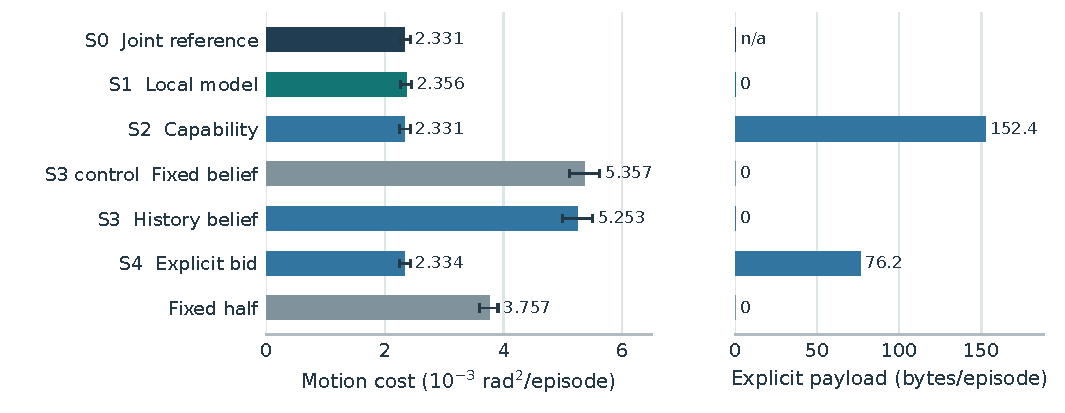
\includegraphics[width=\linewidth]{cost-payload.pdf}
\caption{Deterministic alignment for the first fit, 1,000 matched starts per method. Bars show means and episode bootstrap 95\% intervals for cost. Centralized information is not a comparable message payload. S3's fixed-belief control uses the same solver without history.}
\label{fig:payload}
\end{figure}

\subsection{What the experiments cover}
The completed deterministic benchmark has 23,456 episodes, including 20,000 core episodes. It covers one-arm allocations, fixed half, S0--S4 variants, and selected robustness conditions. The learned benchmark has 25,280 alignment episodes: 24,000 core runs (four regimes, three independent actor/data fits, two sensing modes, 1,000 matched held-out starts) and 1,280 stress runs. The 1,216 contact trials are separate: 128 starts per main condition and 32 matched starts per stress condition. A corrected contact implementation preserves Bullet state during IK; earlier contact diagnostic runs are excluded from these totals.

The principal alignment distribution uses feasible fine offsets within $\pm8$\,mm per lateral axis and $\pm0.18$\,rad in yaw (about $10.3^\circ$), not the proposal's wider target range. Separate camera checks cover feasible wider corners. The smaller stress panels include observation noise, delayed and dropped messages, unequal arm limits, tighter and looser tolerances, history length, and message precision. Neural RGB occlusion is tested separately. Changing history and comparing a fixed-belief control test predictor usefulness indirectly; we did not sweep externally prescribed prediction accuracy or repeat the full S0 comparison under every impairment. Paired intervals resample common starts; they do not substitute for independent fits or justify extrapolation beyond the tested range.

\clearpage
\subsection{Learned alignment and the cost of sensing}
Neural RGB achieved \RgbAlignRange\% alignment success across the 12 actor/regime fits. The same actors with ground-truth observations each aligned on 1,000/1,000 starts, typically with fewer commands and less squared motion. Table~\ref{tab:alignment} holds the actor fixed within each PPO row, isolating the sensing change. Under matched GT sensing, learned actors used fewer commands than fixed half, but all twelve used more squared motion. Useful alignment therefore does not establish a learning advantage. Comparisons between PPO regimes also change the fitted policy, not information alone.

\begin{table}[!ht]
\centering
\caption{Alignment on 1,000 matched test cases per entry for the first fit. Costs are in $10^{-3}$\,rad$^2$/episode; success is in percent. Compare GT and RGB within a PPO row for sensing, or GT columns across controller families. Dashes denote unevaluated RGB counterparts in this alignment benchmark.}
\begin{tabular}{@{}lrrrr@{}}
\toprule
& \multicolumn{2}{c}{Ground truth (GT)} & \multicolumn{2}{c}{Neural RGB} \\
\cmidrule(lr){2-3}\cmidrule(l){4-5}
Controller & Success & Cost & Success & Cost \\ \midrule
\AlignmentRows
\bottomrule
\end{tabular}
\label{tab:alignment}
\end{table}

\subsection{Transfer from visual alignment to insertion}
Across six learned RGB open-hole conditions, including the alternate S1 fits, insertion success ranged from \LearnedContactRange\%. Fixed-half RGB inserted on \HalfInserted/128 starts and S1 with true error on \TruthInserted/128. Holding the S1 actor fixed, RGB minus ground truth was \ContactDiff{} percentage points (paired 95\% interval [\ContactDiffCI]). A common failure was an estimated alignment that passed the vision gate but failed the measured yaw check before descent. There was no privileged correction fallback. All four first-fit learned RGB policies cost more than fixed-half RGB in the contact study, where controllers faced the same initial states; the paired cost intervals were above zero. The motion-cost comparison includes failures and measures endpoint joint displacement, not energy.

\begin{figure}[!ht]
\centering
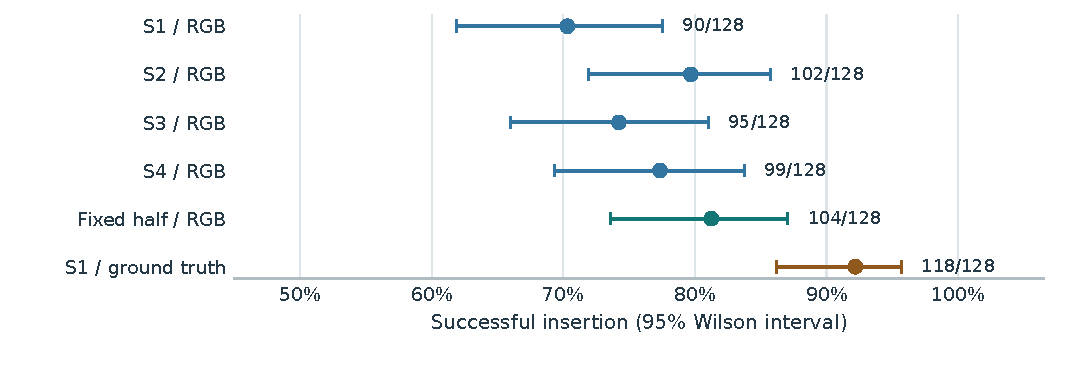
\includegraphics[width=\linewidth]{insertion-success.pdf}
\caption{Open-hole insertion on 128 matched starts per fit-0 condition. Points and Wilson intervals describe insertion, not the earlier alignment benchmark. Only the S1 RGB/ground-truth contrast holds the actor fixed.}
\label{fig:contact}
\end{figure}

\clearpage
\subsection{Where insertion failures occur}
Table~\ref{tab:failures} classifies every main open-hole trial by the stage at which it ended. Among the six learned RGB conditions, \LearnedPreFail{} trials failed before descent, \LearnedDescentFail{} during descent and \LearnedHoldFail{} during the hold. These are pooled counts across different fitted policies, not 768 independent model fits. Of the \LearnedPreFail{} pre-descent failures, \LearnedPoseReject{} were measured-pose rejections after visual alignment and \LearnedVisionReject{} failed the estimated-alignment gate. The separate alignment benchmark's high success therefore does not imply an equally high chance of completing dynamic assembly.

\begin{table}[!ht]
\centering
\caption{Main open-hole outcomes, excluding blocked and stress controls. Failure columns are mutually exclusive. A nonempty descent trace marks descent; a terminal-hold failure takes precedence. Counts, IDs and reasons are included in the bundle.}
\begin{tabular}{@{}lrrrrr@{}}
\toprule
Controller / sensing & N & Before descent & Descent & Hold & Inserted \\ \midrule
\FailureRows
\bottomrule
\end{tabular}
\label{tab:failures}
\end{table}

\subsection{Jam detection and retraction}
The blocked controls produced \BlockedInserted/\BlockedN{} false insertions and \BlockedReleased/\BlockedTried{} released retractions; the other starts were rejected before descent. Only \OpenReleased/\OpenTried{} attempted open-hole retractions released. Thus a controlled blockage verifies one jam response, not universal recovery. Figure~\ref{fig:traces} shows an actual paired validation replay: the open case reaches 20.43\,mm, while the blocked case stalls near the setpoint and retracts to 14.19\,mm with zero residual normal force.

\begin{figure}[!ht]
\centering
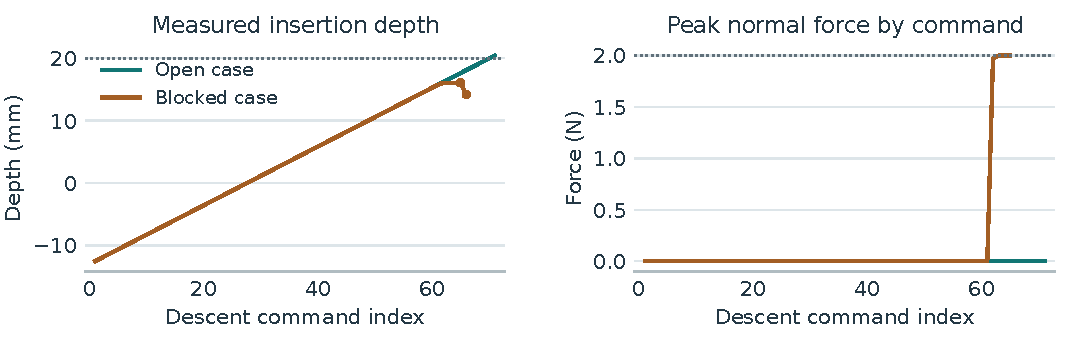
\includegraphics[width=\linewidth]{contact-traces.pdf}
\caption{Paired open/blocked replay with the same S1 RGB actor. Dotted lines mark the 20\,mm depth goal and 2\,N setpoint; the dashed final segment is retraction, not another descent. Selected traces illustrate behavior rather than population-level safety.}
\label{fig:traces}
\end{figure}

\section{Discussion and conclusion}
A shared convention and useful prior let local allocation approach the myopic joint reference without messaging. Capability removed a small cost gap; history and bids offered other speed/payload tradeoffs. This establishes neither a general minimum-bandwidth requirement nor RL efficiency superiority. Contact trials expose a separate transition from visual alignment to guarded insertion. Fixed grasps, one geometry family and sampled force checks limit hardware or safety conclusions. Future work should test whether learned axial corrections or earlier backoff improve insertion or recovery on matched starts at comparable force and travel limits.

\clearpage
\section{Reproduction}
\textbf{Repository:} \RepositoryLink

The accompanying README gives separate instructions to verify the saved results, run a fresh RGB-to-contact replay, and train or evaluate a fresh model. The bundle contains the held-out starts, source, configuration, selected and latest weights, optimizer and RNG checkpoints, all 12 PPO fit logs, and the vision-adaptation records. The raw episodes and SHA-256 manifest support checking the results without retraining. The report plots come from the recomputed study summaries and the recorded replay telemetry. The stopped contact diagnostics are retained and labeled separately.

The allocation fits use data seeds 311--313 and the PPO fits use model seeds 401--403. Validation uses seed 29 with 24 starts; the alignment test uses seed 101 with 1,000 starts. The contact benchmark uses a 128-start slice of that manifest, unused for contact development, with matched stress subsets. The first fit's late S1 candidate was originally ranked using a color-only RGB comparison; its later matched-neural check is diagnostic and the frozen selection is not changed. Three actor fits share a single vision checkpoint. The 24-image validation set supports model selection only within this setup; no independent vision retraining or validation-size sensitivity study was conducted. Between-actor variability therefore cannot establish robustness to perception training or model selection.

\section{Contributions}
The assignments below are from the idea review. A dash indicates that individual fulfillment has not yet been confirmed in this copy.

\begin{table}[!ht]
\centering\small
\begin{tabularx}{\linewidth}{@{}p{.23\linewidth}Xp{.19\linewidth}@{}}
\toprule
Member & Original assignment & Actual fulfillment \\ \midrule
Gaurav Srivastava & Formal model, simulator, feasibility and allocation baselines. & \GauravStatus \\
Aayush Bundel & Decentralized regimes, teammate prediction and message accounting. & \AayushStatus \\
Laxmidhar Swine & CTDE/MAPPO candidate, training protocol and ablations. & \LaxmidharStatus \\
Roshin Gelasious & Paired experiment design, analysis and robustness checks. & \RoshinStatus \\
\bottomrule
\end{tabularx}
\end{table}

\begin{thebibliography}{9}
\bibitem{xie} L. Xie, H. Yu, Y. Zhao, H. Zhang, Z. Zhou, M. Wang, Y. Wang, and R. Xiong. Learning to Fill the Seam by Vision: Sub-millimeter Peg-in-hole on Unseen Shapes in Real World. \emph{Proceedings of the IEEE International Conference on Robotics and Automation (ICRA)}, 2022. \href{https://arxiv.org/abs/2204.07776}{arXiv:2204.07776}.
\bibitem{sfnsystem} G. Srivastava. \emph{Submillimeter Accuracy Peg In Hole Insertion Using Seam Filling Network}. Single-arm research implementation and experimental study, IIT Gandhinagar. \url{https://single-spider.github.io/SFN/}.
\bibitem{bernstein} D. S. Bernstein, R. Givan, N. Immerman, and S. Zilberstein. The Complexity of Decentralized Control of Markov Decision Processes. \emph{Mathematics of Operations Research}, 27(4):819--840, 2002.
\bibitem{ppo} J. Schulman, F. Wolski, P. Dhariwal, A. Radford, and O. Klimov. Proximal Policy Optimization Algorithms. \emph{arXiv preprint}, 2017. \href{https://arxiv.org/abs/1707.06347}{arXiv:1707.06347}.
\bibitem{mappo} C. Yu et al. The Surprising Effectiveness of PPO in Cooperative Multi-Agent Games. \emph{Advances in Neural Information Processing Systems}, 35, 2022. \href{https://arxiv.org/abs/2103.01955}{arXiv:2103.01955}.
\end{thebibliography}
\end{document}
